\documentclass[12pt,a4paper,onecolumn]{exam}

\usepackage{amsmath}
\usepackage{amsthm}
\usepackage{amssymb}
\usepackage{graphicx}
\usepackage{float}
\usepackage{geometry}
\usepackage{tikz}
\usepackage[skins]{tcolorbox}
\usepackage{listings}
\usepackage{xcolor}
\usepackage{hyperref}
\usepackage{multirow}
\usepackage{adjustbox}
\usepackage{booktabs} 
\usepackage[font=small]{caption}
\usepackage{subcaption}

% --- Code Listing Colors ---
\definecolor{codegreen}{rgb}{0,0.6,0}
\definecolor{codegray}{rgb}{0.5,0.5,0.5}
\definecolor{codepurple}{rgb}{0.58,0,0.82}
\definecolor{backcolour}{rgb}{0.95,0.95,0.92}

% --- Code Listing Style ---
\lstdefinestyle{mystyle}{
    backgroundcolor=\color{backcolour},
    commentstyle=\color{codegreen},
    keywordstyle=\color{magenta},
    numberstyle=\tiny\color{codegray},
    stringstyle=\color{codepurple},
    basicstyle=\ttfamily\footnotesize,
    breaklines=true,
    captionpos=b,
    keepspaces=true,
    numbers=left,
    numbersep=2pt,
    showspaces=false,
    showstringspaces=false,
    showtabs=false,
    tabsize=1
}

\newcommand{\questionheader}[1]{%
  \begin{tcolorbox}[
    enhanced,
    colback=black,
    coltext=white,
    boxrule=0pt,
    fontupper=\Large\bfseries,
    arc=4mm
  ]
  #1
  \end{tcolorbox}%
}


\lstset{style=mystyle, language=Python}

\begin{document}

\begingroup
    \centering
    \LARGE E1 244 Detection and Estimation Theory\\
    \LARGE Assignment 4\\[0.5em]
    \large Dwaipayan Haldar\par
    \large \today\\[0.5em]
\endgroup
\noindent\rule{\textwidth}{0.5pt}
\printanswers
\renewcommand{\solutiontitle}{\noindent\textbf{Ans:}\enspace}

%----------------------------------------------------------------------
\questionheader{Problem 1}
%----------------------------------------------------------------------

\begin{solution}

The state-space model is:
\[
  y_i = x_i + w_i, \quad i = 1, 2, \ldots, N, \quad w_i \sim \mathcal{N}(0,\sigma_w^2),
\]
\[
  x_i = \alpha\, x_{i-1}, \qquad x_0 = \theta \sim \mathcal{N}(0,\sigma^2),
\]
with $\theta$ independent of $w_1, w_2, \ldots, w_N$.

\textbf{(a) MMSE estimate $\hat{\theta}_{\mathrm{MMSE}}$}

Since $x_i = \alpha^i \theta$, the signal at time $i$ is $x_i = \alpha^i\theta$. Therefore:
\[
  p(y_i \mid \theta) \sim \mathcal{N}(\alpha^i\theta,\, \sigma_w^2).
\]
The joint likelihood (observations are conditionally independent given $\theta$) is:
\[
  p(\mathbf{y} \mid \theta) = \frac{1}{(2\pi)^{N/2}\,\sigma_w^N}
    \exp\!\left(-\frac{1}{2\sigma_w^2}\sum_{i=1}^N (y_i - \alpha^i\theta)^2\right).
\]
The prior is $p(\theta) = \frac{1}{\sigma\sqrt{2\pi}}\exp\!\left(-\frac{\theta^2}{2\sigma^2}\right)$.

To compute $p(\mathbf{y}) = \int_{-\infty}^{\infty} p(\mathbf{y}\mid\theta)\,p(\theta)\,d\theta$, we evaluate the non-constant part of the integrand:
\[
  \int_{-\infty}^{\infty}
    \exp\!\left[-\frac{1}{2\sigma_w^2}\!\left(\sum_i y_i^2 + \theta^2\sum_i\alpha^{2i}
      - 2\theta\sum_i \alpha^i y_i\right)\right]
    \exp\!\left(-\frac{\theta^2}{2\sigma^2}\right) d\theta.
\]
Grouping terms and defining:
\[
  A = \frac{\sum_i \alpha^{2i}}{\sigma_w^2} + \frac{1}{\sigma^2}, \qquad
  B = \frac{\sum_i \alpha^i y_i}{\sigma_w^2}, \qquad
  C = \frac{\sum_i y_i^2}{\sigma_w^2},
\]
the integrand becomes $\exp\!\left[-\tfrac{1}{2}(A\theta^2 - 2B\theta + C)\right]$. Completing the square:
\[
  \int_{-\infty}^{\infty}
    \exp\!\left[-\frac{A}{2}\!\left(\theta - \frac{B}{A}\right)^2\right]
    \exp\!\left[-\frac{1}{2}\!\left(C - \frac{B^2}{A}\right)\right] d\theta
  = \sqrt{\frac{2\pi}{A}}\,\exp\!\left[-\frac{1}{2}\!\left(C - \frac{B^2}{A}\right)\right].
\]
Therefore:
\[
  E(\theta \mid \mathbf{y}) = \frac{B}{A}
    = \frac{\displaystyle\frac{\sum_i \alpha^i y_i}{\sigma_w^2}}{\displaystyle\frac{\sum_i \alpha^{2i}}{\sigma_w^2} + \frac{1}{\sigma^2}}
    = \frac{\sum_i \alpha^i y_i}{\sum_i \alpha^{2i} + \dfrac{\sigma_w^2}{\sigma^2}}.
\]
\[
  \boxed{\hat{\theta}_{\mathrm{MMSE}}(\mathbf{y}) = \frac{\sum_{i=1}^N \alpha^i y_i}{\sum_{i=1}^N \alpha^{2i} + \dfrac{\sigma_w^2}{\sigma^2}}.}
\]

\textbf{(b) Recursive LLSE}

Since $\hat{\theta}_{\mathrm{MMSE}}$ is linear in $\mathbf{y}$, it is also the LLSE. We derive it recursively.

\emph{Initialization ($i=1$):}
\[
  \hat{\theta}_1 = l_1\, y_1, \quad
  l_1 = \frac{E[\theta y_1]}{E[y_1^2]}
       = \frac{E[\theta(\alpha\theta + w_1)]}{E[(\alpha\theta+w_1)^2]}
       = \frac{\alpha\sigma^2}{\alpha^2\sigma^2 + \sigma_w^2}.
\]

\emph{Recursive update:}
\[
  \hat{\theta}_i = \hat{\theta}_{i-1} + l_i\, z_i, \quad
  z_i = y_i - \hat{y}_i(y_1,\ldots,y_{i-1}). \tag{1}
\]
Since $y_i = \alpha^i\theta + w_i$ and from LLS properties $\hat{w}_i = 0$ (as $\theta$, $w_i$, and $w_j$ for $i\neq j$ are independent with zero means):
\[
  \hat{y}_i(y_1,\ldots,y_{i-1}) = \alpha^i\hat{\theta}_{i-1},
  \qquad\Rightarrow\qquad
  z_i = y_i - \alpha^i\hat{\theta}_{i-1}.
\]
The gain $l_i = \dfrac{E[\theta\, z_i]}{E[z_i^2]}$. Denoting the error $e_i = \theta - \hat{\theta}_i$:

\[
  E[\theta\, z_i]
    = E\!\left[\theta(y_i - \alpha^i\hat{\theta}_{i-1})\right]
    = E\!\left[\alpha^i\theta(\theta - \hat{\theta}_{i-1}) - \theta w_i\right]
    = \alpha^i E[e_{i-1}^2]
\]
(using $E[\theta w_i]=0$ and orthogonality of error and estimate).

\[
  E[z_i^2]
    = E\!\left[(\alpha^i e_{i-1} + w_i)^2\right]
    = \alpha^{2i} E[e_{i-1}^2] + \sigma_w^2
\]
(using $E[e_{i-1} w_i]=0$, since $e_{i-1}$ depends on $y_1,\ldots,y_{i-1}$ which are independent of $w_i$).

Therefore:
\[
  l_i = \frac{\alpha^i E[e_{i-1}^2]}{\alpha^{2i} E[e_{i-1}^2] + \sigma_w^2}.
\]
The mean-squared error evolves as:
\begin{align*}
  E[e_i^2]
    &= E\!\left[(e_{i-1} - l_i(\alpha^i e_{i-1} + w_i))^2\right]
     = (1 - l_i\alpha^i)^2 E[e_{i-1}^2] + l_i^2\,\sigma_w^2 \\
    &= \frac{\sigma_w^2\, E[e_{i-1}^2]}{\alpha^{2i} E[e_{i-1}^2] + \sigma_w^2}.
\end{align*}
Define $K_i = \dfrac{\sigma_w^2}{E[e_i^2]}$ with $K_0 = \dfrac{\sigma_w^2}{\sigma^2}$ (since $\hat{\theta}_0=0 \Rightarrow E[e_0^2]=\sigma^2$). Then:
\[
  K_i = \frac{\sigma_w^2(\alpha^{2i} E[e_{i-1}^2] + \sigma_w^2)}{\sigma_w^2\, E[e_{i-1}^2]}
      = \alpha^{2i} + K_{i-1}.
\]
Substituting back into~(1):
\[
  \hat{\theta}_i
    = (1 - l_i\alpha^i)\hat{\theta}_{i-1} + l_i\, y_i
    = \frac{\sigma_w^2}{\alpha^{2i} E[e_{i-1}^2]+\sigma_w^2}\,\hat{\theta}_{i-1}
      + \frac{E[e_{i-1}^2]\,\alpha^i}{\alpha^{2i} E[e_{i-1}^2]+\sigma_w^2}\, y_i.
\]
Multiplying numerator and denominator by $K_i$:
\[
  \boxed{\hat{\theta}_i = K_i^{-1}\!\left[K_{i-1}\,\hat{\theta}_{i-1} + \alpha^i\, y_i\right].}
\]

\textbf{(c) Behavior of $e_i$}

From part~(b), $K_i = K_{i-1} + \alpha^{2i}$, so unrolling:
\[
  K_i = K_0 + \sum_{k=1}^{i}\alpha^{2k}
      = \frac{\sigma_w^2}{\sigma^2} + \sum_{k=1}^{i}\alpha^{2k}.
\]
Therefore:
\[
  \frac{\sigma_w^2}{e_i} = \frac{\sigma_w^2}{\sigma^2} + \sum_{k=1}^{i}\alpha^{2k}
  \qquad\Rightarrow\qquad
  e_i = \frac{1}{\dfrac{1}{\sigma^2} + \dfrac{1}{\sigma_w^2}\displaystyle\sum_{k=0}^{i}\alpha^{2k}}.
\]
\begin{itemize}
  \item When $|\alpha| \geq 1$: $\sum_{k=0}^{i}\alpha^{2k} \to \infty$, so $e_i \to 0$ as $i\to\infty$.
  \item When $|\alpha| < 1$: $\sum_{k=0}^{\infty}\alpha^{2k} = \dfrac{1}{1-\alpha^2}$, so
    \[
      e_i \;\xrightarrow{i\to\infty}\; \frac{1}{\dfrac{1}{\sigma^2} + \dfrac{\alpha^2}{\sigma_w^2(1-\alpha^2)}}.
    \]
\end{itemize}

\end{solution}

%----------------------------------------------------------------------
\questionheader{Problem 2}
%----------------------------------------------------------------------

\begin{solution}

\textbf{(a) MMSE estimate of $x_2$ given $x_1$}

Given:
\[
  \begin{bmatrix} x_1 \\ x_2 \end{bmatrix}
  \sim \mathcal{N}\!\left(
    \begin{bmatrix} 0 \\ 0 \end{bmatrix},\,
    \begin{bmatrix} \sigma_{x_1}^2 & \mathrm{cov}(x_1,x_2) \\
                    \mathrm{cov}(x_1,x_2) & \sigma_{x_2}^2 \end{bmatrix}
  \right).
\]
From the conditional Gaussian result:
\[
  x_2 \mid x_1 \sim \mathcal{N}\!\left(
    \frac{\mathrm{cov}(x_1,x_2)}{\sigma_{x_1}^2}\,x_1,\;
    \sigma_{x_2}^2 - \frac{[\mathrm{cov}(x_1,x_2)]^2}{\sigma_{x_1}^2}
  \right).
\]
Therefore:
\[
  \hat{x}_2(x_1) = E[x_2 \mid x_1] = \frac{\mathrm{cov}(x_1,x_2)}{\sigma_{x_1}^2}\,x_1.
\]
Since the MMSE estimate is linear in $x_1$, MMSE $=$ LLS in this case.

\textbf{(b) Cost and singular $R_x$}

\[
  C(x_2,\hat{x}_2) = E[(x_2 - \hat{x}_2)^2]
    = E_{x_1}[\mathrm{Var}(x_2 \mid x_1)]
    = \sigma_{x_2}^2 - \frac{[\mathrm{cov}(x_1,x_2)]^2}{\sigma_{x_1}^2}.
\]
Now $C(x_2,\hat{x}_2) = 0 \iff \sigma_{x_1}^2\,\sigma_{x_2}^2 = [\mathrm{cov}(x_1,x_2)]^2$, which is exactly the condition for $R_x$ to be singular.

\textbf{(c) Perfect estimation when $R_x$ is singular}

Suppose we want to estimate $x_1$ given $x_2, \ldots, x_N$ (WLOG). Let $\mathbf{x}' = [x_2,\ldots,x_N]^\top$. The LLS estimate is:
\[
  \hat{x}_1 = \Sigma_{x_1 \mathbf{x}'}\,\Sigma_{\mathbf{x}'\mathbf{x}'}^{-1}\,\mathbf{x}',
\]
with cost:
\[
  C(x_1,\hat{x}_1) = \sigma_{x_1 x_1} - \Sigma_{x_1\mathbf{x}'}\,\Sigma_{\mathbf{x}'\mathbf{x}'}^{-1}\,\Sigma_{\mathbf{x}'x_1}.
\]
Since $R_x \succeq 0$ and $\det(R_x) = 0$, using the Schur complement formula:
\[
  \det(R_x) = \det(\Sigma_{\mathbf{x}'\mathbf{x}'}) \cdot
    \left(\sigma_{x_1 x_1} - \Sigma_{x_1\mathbf{x}'}\,\Sigma_{\mathbf{x}'\mathbf{x}'}^{-1}\,\Sigma_{\mathbf{x}'x_1}\right) = 0.
\]
This implies $\sigma_{x_1 x_1} - \Sigma_{x_1\mathbf{x}'}\,\Sigma_{\mathbf{x}'\mathbf{x}'}^{-1}\,\Sigma_{\mathbf{x}'x_1} = 0$, i.e.\ $C(x_1,\hat{x}_1) = 0$.

Hence \textbf{perfect estimation is possible}.

\end{solution}

%----------------------------------------------------------------------
\questionheader{Problem 3}
%----------------------------------------------------------------------

\begin{solution}

Setup: $y = x + w$, $x \sim \mathrm{Uniform}(0,\alpha)$, $w \sim \mathrm{Exp}(\lambda)$, independent.

\textbf{(a)(i) Conditional pdf $f(y \mid x)$}

\[
  P(y \leq t \mid x) = P(w \leq t - x \mid x) = F_w(t-x).
\]
\[
  f(y \mid x) = f_w(y - x) = \lambda e^{-\lambda(y-x)}\,\mathbf{1}_{\{y \geq x\}}.
\]
Support: $y \geq x$.

\textbf{(a)(ii) Marginal pdf $f(y)$}

\[
  f(y) = \int_{-\infty}^{\infty} f(y \mid x)\,f(x)\,dx
        = \frac{\lambda}{\alpha}\int_0^{\alpha} e^{-\lambda(y-x)}\,\mathbf{1}_{\{y \geq x\}}\,dx.
\]
\textit{Case 1: $0 \leq y \leq \alpha$}
\[
  f(y) = \frac{\lambda}{\alpha}\int_0^{y} e^{-\lambda(y-x)}\,dx
        = \frac{\lambda}{\alpha}\,e^{-\lambda y}\,\frac{e^{\lambda y}-1}{\lambda}
        = \frac{1}{\alpha}(1 - e^{-\lambda y}).
\]
\textit{Case 2: $y \geq \alpha$}
\[
  f(y) = \frac{\lambda}{\alpha}\int_0^{\alpha} e^{-\lambda(y-x)}\,dx
        = \frac{\lambda}{\alpha}\,e^{-\lambda y}\,\frac{e^{\lambda\alpha}-1}{\lambda}
        = e^{-\lambda y}\,\frac{e^{\lambda\alpha}-1}{\alpha}.
\]
\[
  f(y) = \begin{cases}
    0 & y < 0,\\
    \dfrac{1}{\alpha}(1 - e^{-\lambda y}) & 0 \leq y \leq \alpha,\\[6pt]
    e^{-\lambda y}\,\dfrac{e^{\lambda\alpha}-1}{\alpha} & y \geq \alpha.
  \end{cases}
\]

\textbf{(a)(iii) Posterior pdf $f(x \mid y)$}

\[
  f(x \mid y) = \frac{f(y \mid x)\,f(x)}{f(y)}
    = \frac{\lambda\,e^{\lambda x}\,\mathbf{1}_{\{0 \leq x \leq \min(y,\alpha)\}}}
           {(e^{\lambda y}-1)\,\mathbf{1}_{\{0 \leq y \leq \alpha\}} + (e^{\lambda\alpha}-1)\,\mathbf{1}_{\{y \geq \alpha\}}}.
\]
Support: $0 \leq x \leq \min(y,\alpha)$.

\textbf{(b) MAP estimate}

\[
  \hat{x}_{\mathrm{MAP}} = \operatorname*{arg\,max}_{x}\, f(x \mid y).
\]
Since $\lambda e^{\lambda x}$ is increasing in $x$ for $\lambda > 0$, the maximum is at the right boundary of the support:
\[
  \boxed{\hat{x}_{\mathrm{MAP}} = \min(y,\alpha).}
\]

\textbf{(c) MAE (Median) estimate}

$\hat{x}_{\mathrm{MAE}}$ is the median of $f(x\mid y)$, satisfying $\int_{\hat{x}_{\mathrm{MAE}}}^{\min(y,\alpha)} f(x\mid y)\,dx = \tfrac{1}{2}$.

\textit{Case 1: $\min(y,\alpha) = y$ (i.e.\ $y \leq \alpha$)}
\[
  \int_{\hat{x}_{\mathrm{MAE}}}^{y} \frac{\lambda e^{\lambda x}}{e^{\lambda y}-1}\,dx = \frac{1}{2}
  \implies \frac{e^{\lambda y} - e^{\lambda\hat{x}_{\mathrm{MAE}}}}{e^{\lambda y}-1} = \frac{1}{2}
  \implies \hat{x}_{\mathrm{MAE}} = \frac{1}{\lambda}\ln\frac{e^{\lambda y}+1}{2}.
\]

\textit{Case 2: $\min(y,\alpha) = \alpha$ (i.e.\ $y \geq \alpha$)}
\[
  \int_{\hat{x}_{\mathrm{MAE}}}^{\alpha} \frac{\lambda e^{\lambda x}}{e^{\lambda\alpha}-1}\,dx = \frac{1}{2}
  \implies 2(e^{\lambda\alpha} - e^{\lambda\hat{x}_{\mathrm{MAE}}}) = e^{\lambda\alpha}-1
  \implies \hat{x}_{\mathrm{MAE}} = \frac{1}{\lambda}\ln\frac{e^{\lambda\alpha}+1}{2}.
\]
Combining:
\[
  \boxed{\hat{x}_{\mathrm{MAE}} = \frac{1}{\lambda}\ln\frac{e^{\lambda\min(y,\alpha)}+1}{2}.}
\]

\textbf{(d) MMSE estimate}

\[
  \hat{x}_{\mathrm{MMSE}} = E[x \mid y]
    = \int_0^{\min(y,\alpha)} x \cdot \frac{\lambda e^{\lambda x}}{e^{\lambda\min(y,\alpha)}-1}\,dx.
\]
Let $b = \lambda\min(y,\alpha)$ and substitute $t = \lambda x$:
\[
  = \frac{1}{\lambda^2(e^b-1)}\int_0^b t\,e^t\,dt
  = \frac{1}{\lambda^2(e^b-1)}\bigl[te^t - e^t\bigr]_0^b
  = \frac{1}{\lambda^2(e^b-1)}\bigl[e^b(b-1)+1\bigr].
\]
\[
  \boxed{\hat{x}_{\mathrm{MMSE}} = \frac{e^{\lambda\min(y,\alpha)}\bigl(\lambda\min(y,\alpha)-1\bigr)+1}{\lambda\bigl(e^{\lambda\min(y,\alpha)}-1\bigr)}.}
\]

\end{solution}

%----------------------------------------------------------------------
\questionheader{Problem 4}
%----------------------------------------------------------------------

\begin{solution}

The system model is the Gauss--Markov process:
\[
  x_{i+1} = A\,x_i + B\,w_i, \qquad y_i = C\,x_i + v_i,
\]
where $w_i \sim \mathcal{N}(0, W)$ and $v_i \sim \mathcal{N}(0, V)$ are independent process and measurement noise, and $x_0 \sim \mathcal{N}(\hat{x}_0, \Sigma_0)$.\\

\textbf{(a) Helper function: sampling from a multivariate Gaussian}

To simulate the state and measurement trajectories, we need to draw samples from multivariate normal distributions at each time step. The following one-line function wraps NumPy's sampler and returns a column vector:

\begin{lstlisting}
import numpy as np

def sample_from_multivariate_normal(mean, cov):
    return np.random.multivariate_normal(mean, cov, 1).T
\end{lstlisting}

\textbf{Explanation.}
\texttt{np.random.multivariate\_normal(mean, cov, 1)} draws one sample from $\mathcal{N}(\texttt{mean}, \texttt{cov})$ and returns a row vector of shape $(1, n)$. Transposing with \texttt{.T} converts it to a column vector of shape $(n, 1)$, which matches the standard state-space convention $x_i \in \mathbb{R}^n$. \\

\textbf{(b) Kalman Filter Trajectory: True State vs.\ Filtered Estimate}

The Kalman filter was run for $K=100$ time steps with measurement noise variance $V \in \{0.1, 0.2, \ldots, 0.9\}$ (the case $V=1.0$ is omitted here as it is covered in part~(c)). Figure~\ref{fig:kf_traj} shows the first component $x_{k,1}$ of the true state alongside the filtered estimate $\hat{x}_{k|k-1,1}$ for each value of $V$.

\begin{figure}[H]
  \centering
  % Row 1
  \begin{subfigure}[b]{0.31\textwidth}
    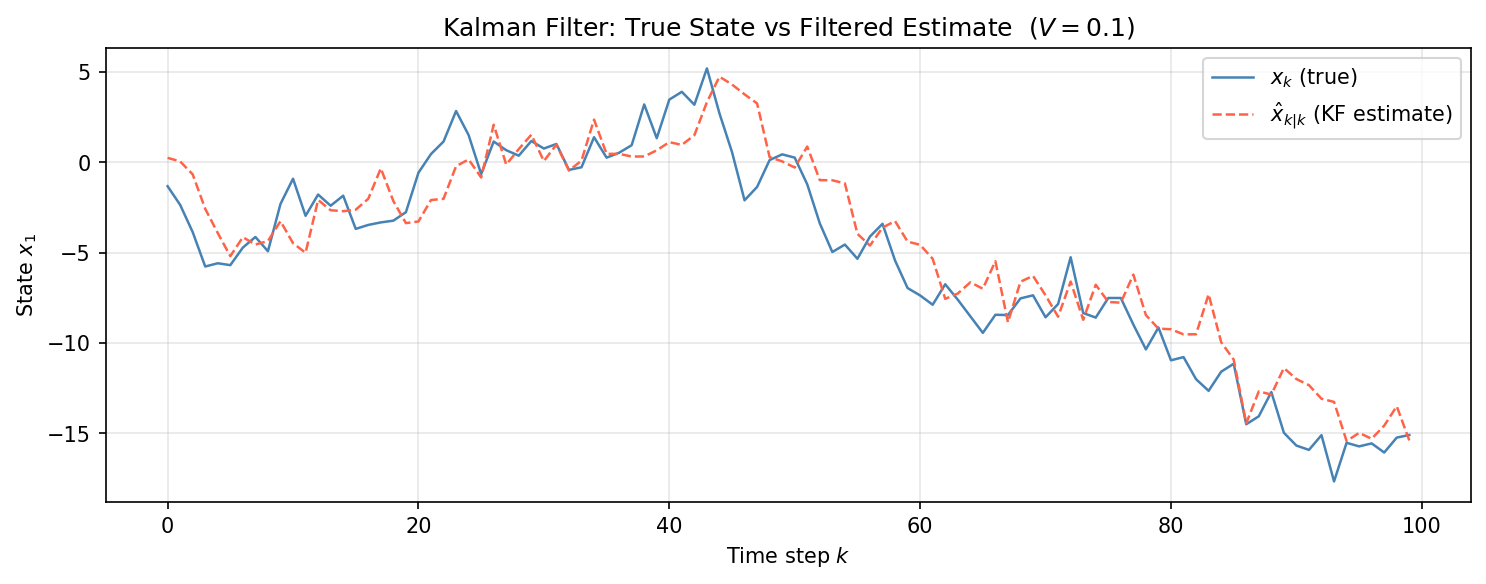
\includegraphics[width=\textwidth]{output/KF_trajectory_v=0.1.png}
    \caption*{$V=0.1$}
  \end{subfigure}\hfill
  \begin{subfigure}[b]{0.31\textwidth}
    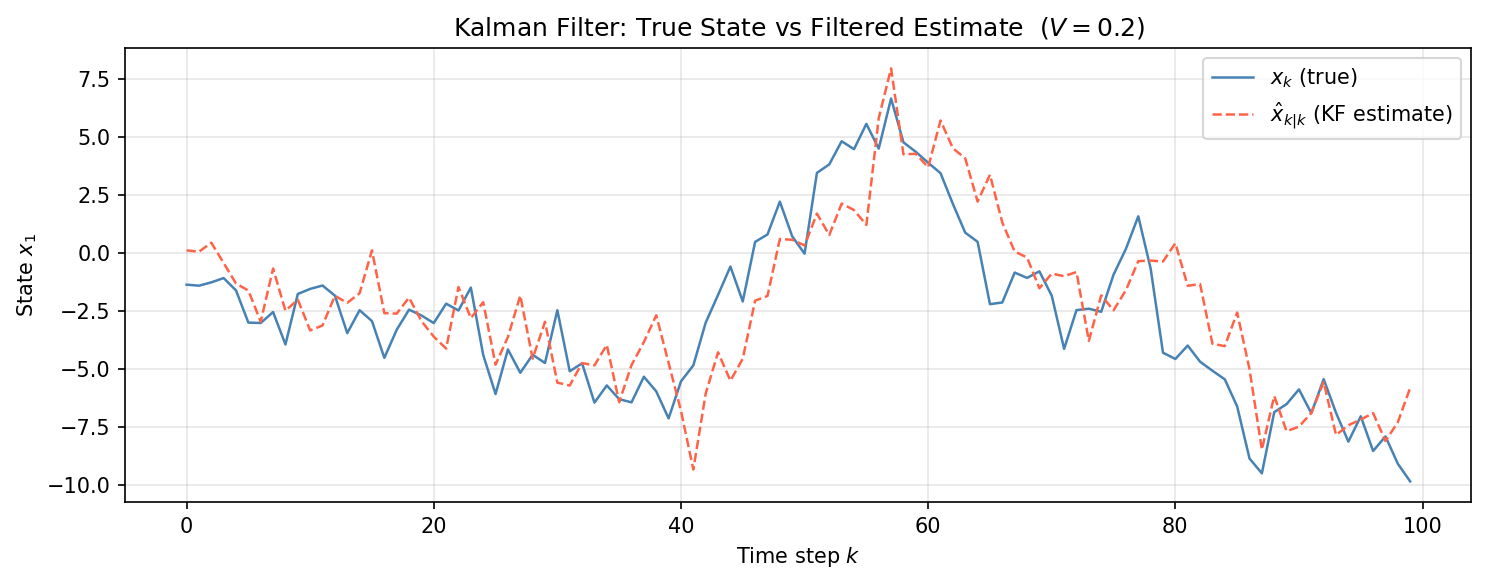
\includegraphics[width=\textwidth]{output/KF_trajectory_v=0.2.png}
    \caption*{$V=0.2$}
  \end{subfigure}\hfill
  \begin{subfigure}[b]{0.31\textwidth}
    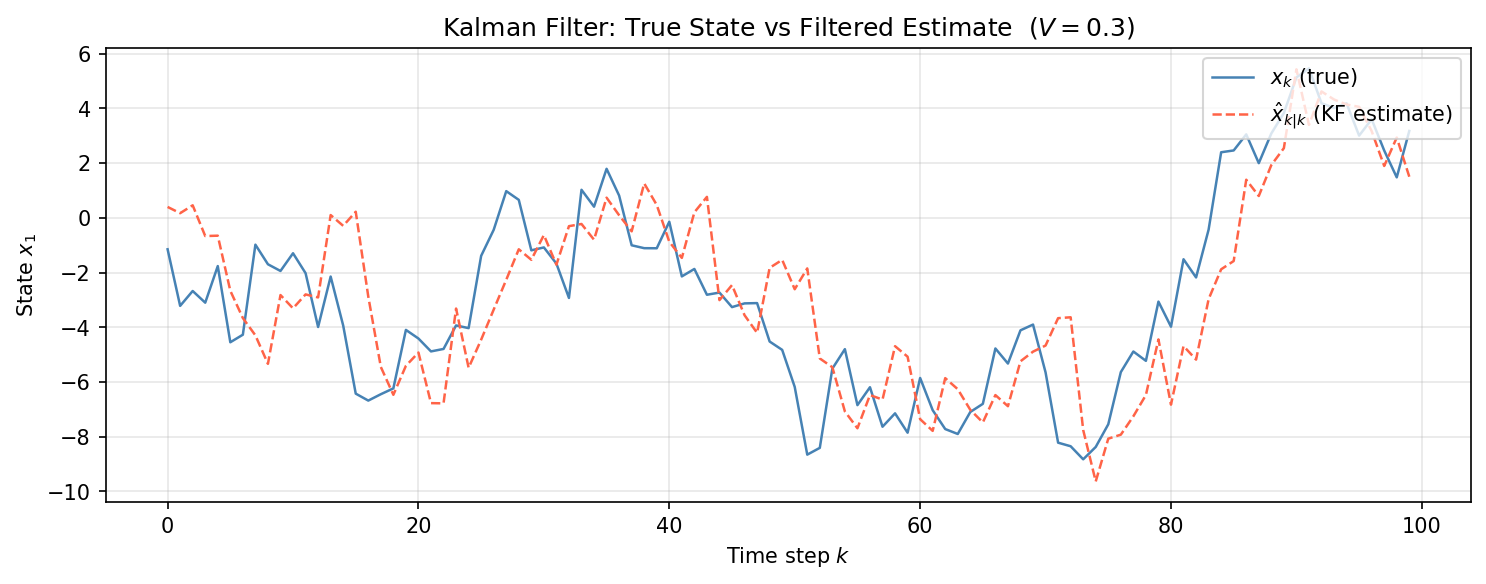
\includegraphics[width=\textwidth]{output/KF_trajectory_v=0.3.png}
    \caption*{$V=0.3$}
  \end{subfigure}
  \\[0.8em]
  % Row 2
  \begin{subfigure}[b]{0.31\textwidth}
    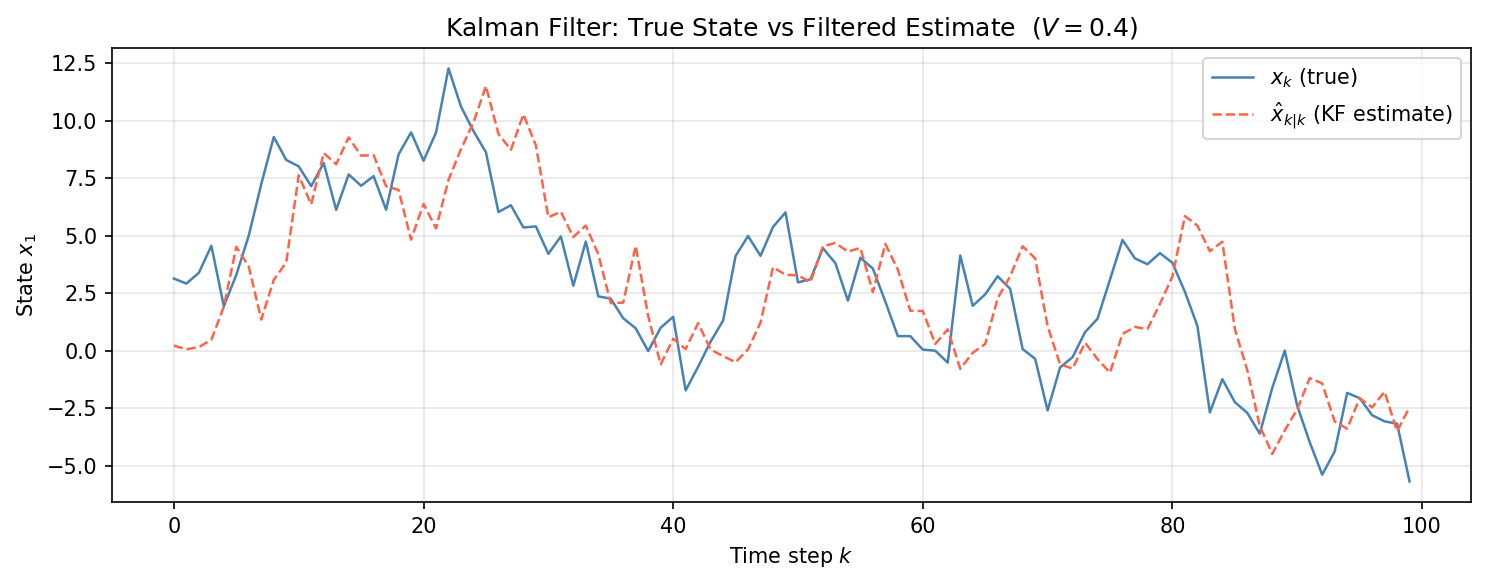
\includegraphics[width=\textwidth]{output/KF_trajectory_v=0.4.png}
    \caption*{$V=0.4$}
  \end{subfigure}\hfill
  \begin{subfigure}[b]{0.31\textwidth}
    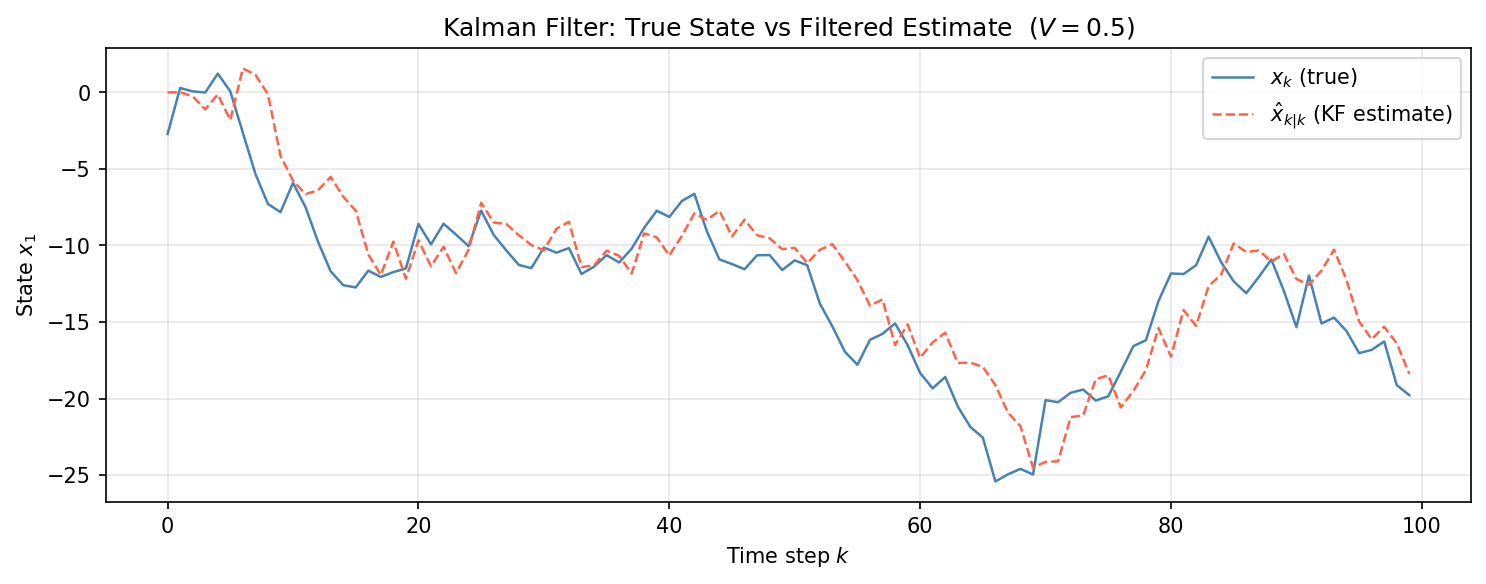
\includegraphics[width=\textwidth]{output/KF_trajectory_v=0.5.png}
    \caption*{$V=0.5$}
  \end{subfigure}\hfill
  \begin{subfigure}[b]{0.31\textwidth}
    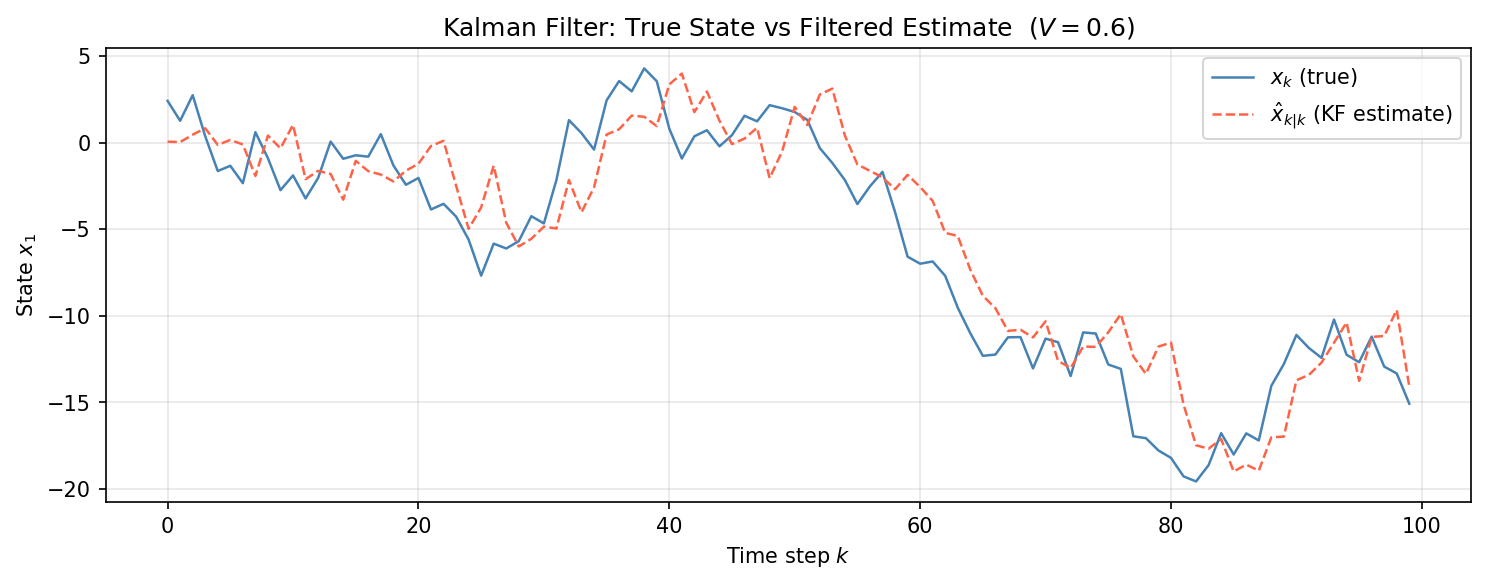
\includegraphics[width=\textwidth]{output/KF_trajectory_v=0.6.png}
    \caption*{$V=0.6$}
  \end{subfigure}
  \\[0.8em]
  % Row 3
  \begin{subfigure}[b]{0.31\textwidth}
    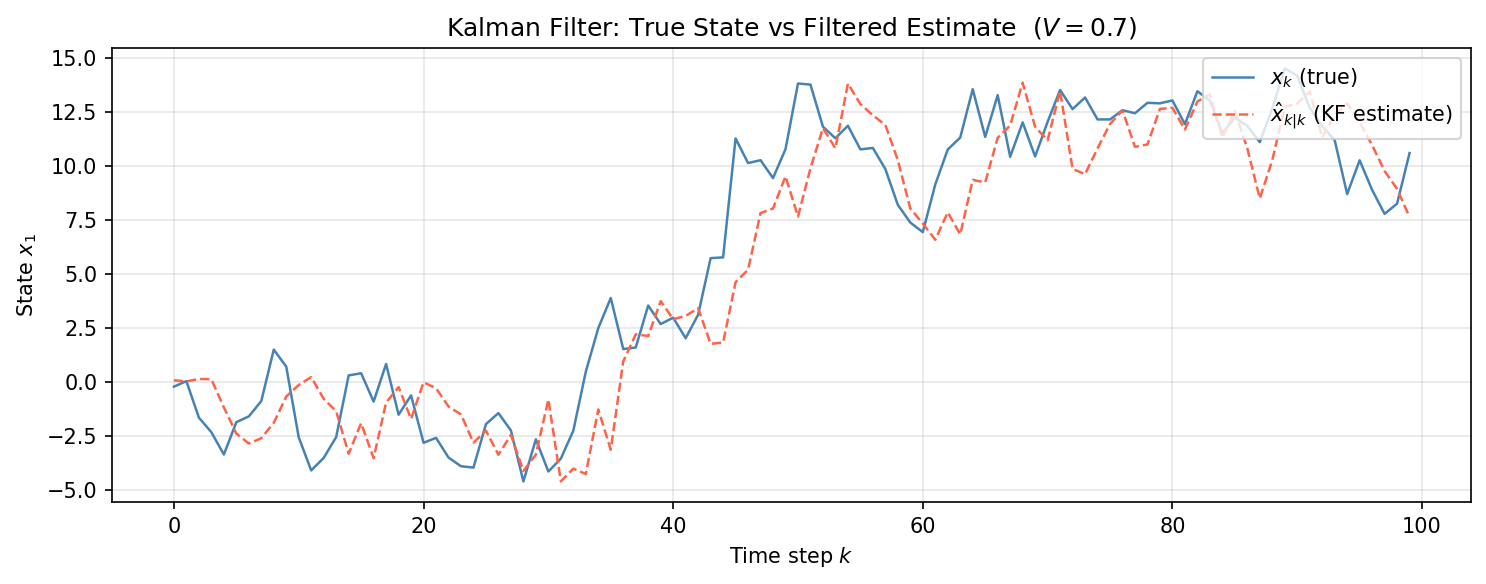
\includegraphics[width=\textwidth]{output/KF_trajectory_v=0.7.png}
    \caption*{$V=0.7$}
  \end{subfigure}\hfill
  \begin{subfigure}[b]{0.31\textwidth}
    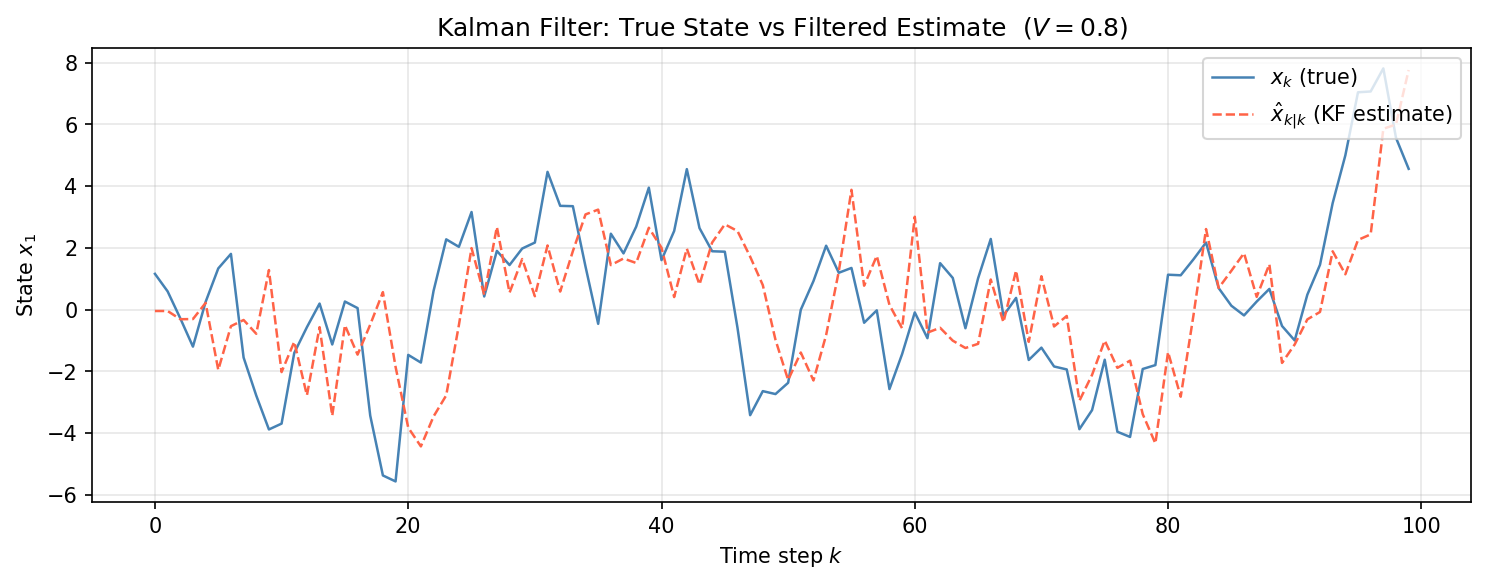
\includegraphics[width=\textwidth]{output/KF_trajectory_v=0.8.png}
    \caption*{$V=0.8$}
  \end{subfigure}\hfill
  \begin{subfigure}[b]{0.31\textwidth}
    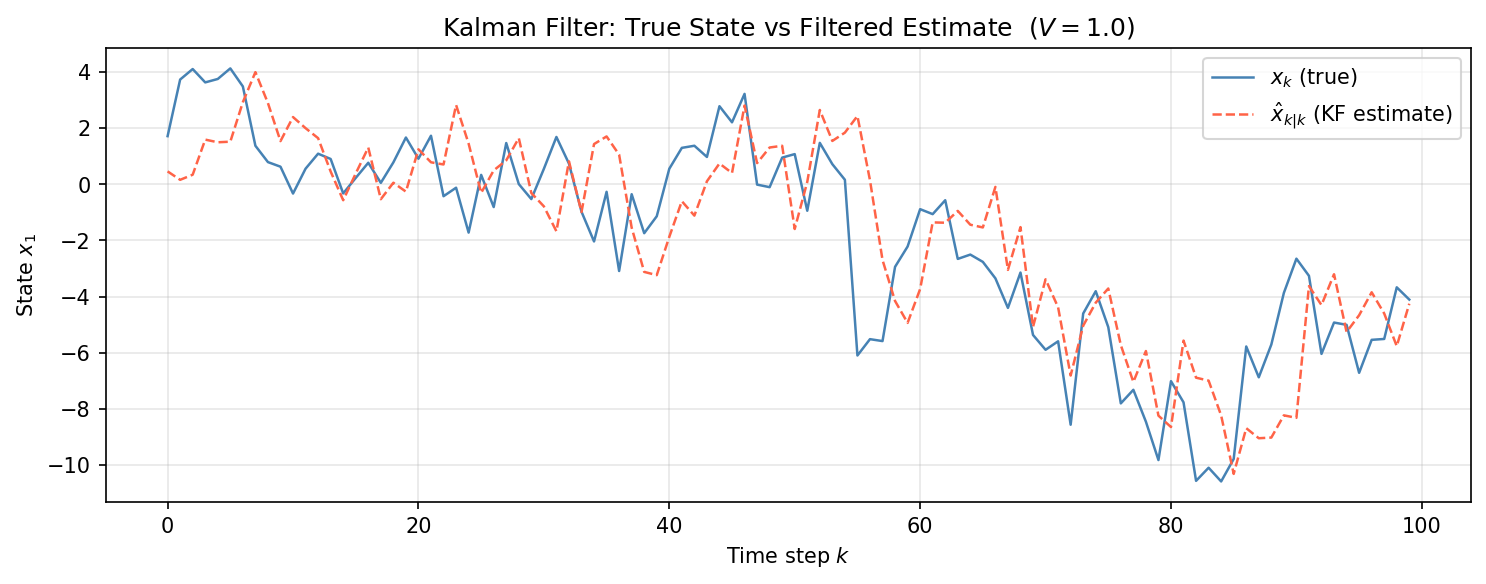
\includegraphics[width=\textwidth]{output/KF_trajectory_v=1.0.png}
    \caption*{$V=1$}
  \end{subfigure}
  \caption{True state $x_{k,1}$ (blue) vs.\ KF predicted estimate $\hat{x}_{k|k-1,1}$ (red dashed) for varying measurement noise variance $V$.}
  \label{fig:kf_traj}
\end{figure}

\textbf{Discussion.} As $V$ decreases, the measurement noise decreases and the measurements become more informative. Consequently, the filter trusts the observations more and the predicted estimate tracks the true state more closely. At small $V$ (e.g.\ $V=0.1$), the two curves are nearly indistinguishable, while at large $V$ (e.g.\ $V=1$) the estimate lags noticeably behind the true state. \\ 

\vspace{1.5em}
\textbf{(c) Theoretical vs.\ Empirical Error Covariance}

The theoretical prediction error covariance $R_{k|k-1}$ is propagated via the Riccati recursion:
\[
  R_{k|k-1} = A\,R_{k-1|k-1}\,A^\top + B\,W\,B^\top, \qquad
  R_{k|k} = R_{k|k-1} - L_k\,C\,R_{k|k-1},
\]
and compared against the empirical trace obtained from $M=100{,}000$ independent Monte Carlo runs at $V=1$.

The predicted error covariance is defined as:
\[
  R_{k|k-1} = E\!\left[(x_k - \hat{x}_{k|k-1})(x_k - \hat{x}_{k|k-1})^\top\right],
\]
so its trace equals the total mean squared prediction error:
\[
  \mathrm{tr}(R_{k|k-1}) = E\!\left[\|x_k - \hat{x}_{k|k-1}\|^2\right].
\]
To estimate this empirically, the KF is run $M$ times independently. On the $i$-th run the prediction error at time $k$ is $e_k^{(i)} = x_k^{(i)} - \hat{x}_{k|k-1}^{(i)}$, and the sample mean
\[
  \widehat{\mathrm{tr}(R_{k|k-1})} = \frac{1}{M}\sum_{i=1}^{M}\left(e_k^{(i)}\right)^\top e_k^{(i)}
\]
converges to $\mathrm{tr}(R_{k|k-1})$ as $M\to\infty$ by the Law of Large Numbers.

\begin{figure}[H]
  \centering
  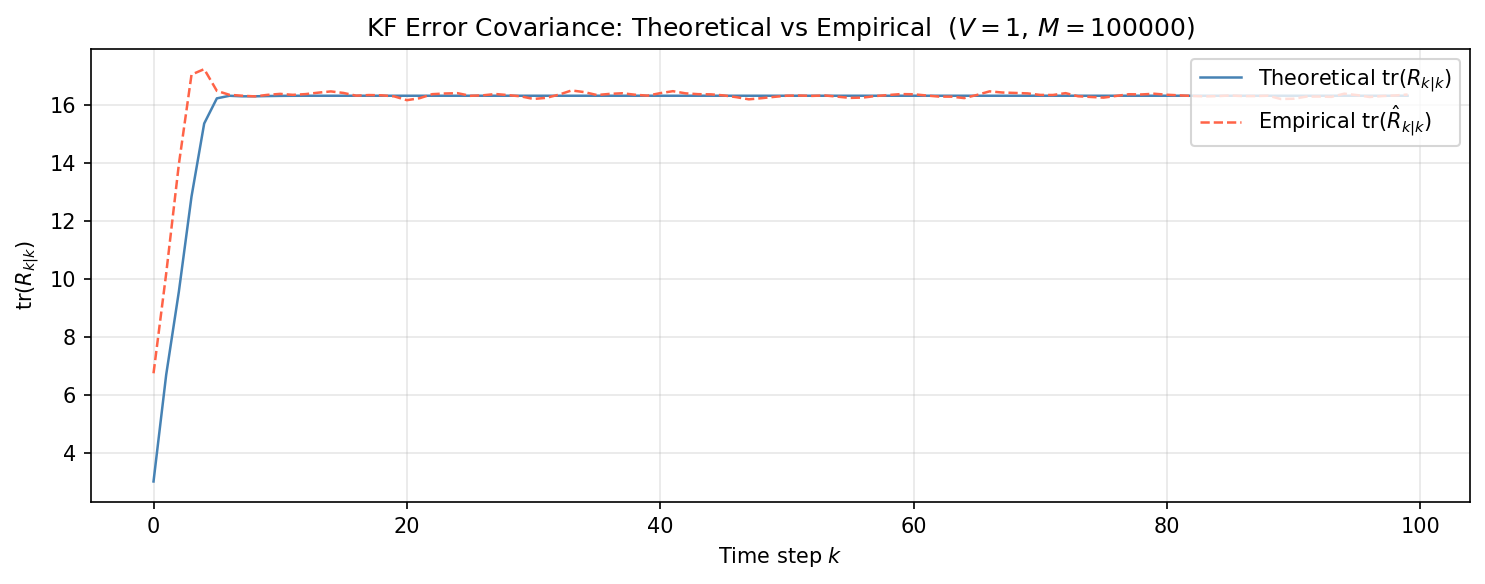
\includegraphics[width=0.8\textwidth]{output/KF_covariance_v=1_M=100000.png}
  \caption{Theoretical $\mathrm{tr}(R_{k|k-1})$ (blue) vs.\ empirical $\mathrm{tr}(\hat{R}_{k|k-1})$ (red dashed) for $V=1$, $M=100{,}000$.}
  \label{fig:kf_cov}
\end{figure}

\textbf{Discussion.} The Riccati recursion converges to the steady-state solution of the algebraic Riccati equation (ARE), so $\mathrm{tr}(R_{k|k-1})$ saturates after a few dozen time steps. The empirical trace closely follows the theoretical curve, with the match improving as $k$ increases because the initial transient (sensitive to the choice of $\Sigma_0$) dies out and the filter reaches its steady state.

\end{solution}

%----------------------------------------------------------------------
\questionheader{Problem 5}
%----------------------------------------------------------------------

\begin{solution}

\textbf{(a) Linearity of LLS}

From the LLS derivation, with $\beta = A_1\theta_1 + A_2\theta_2 + c$:
\[
  \hat{\beta}_{\mathrm{LLS}}(\mathbf{y}) = \mu_\beta + R_{\beta y}\,R_{yy}^{-1}(\mathbf{y}-\mu_y).
\]
\[
  \mu_\beta = A_1\mu_{\theta_1} + A_2\mu_{\theta_2} + c.
\]
\begin{align*}
  R_{\beta y}
    &= E[(\beta-\mu_\beta)(\mathbf{y}-\mu_y)^\top] \\
    &= E\!\left[(A_1(\theta_1-\mu_{\theta_1}) + A_2(\theta_2-\mu_{\theta_2}))(\mathbf{y}-\mu_y)^\top\right] \\
    &= A_1 R_{\theta_1 y} + A_2 R_{\theta_2 y}.
\end{align*}
Therefore:
\begin{align*}
  \hat{\beta}_{\mathrm{LLS}}(\mathbf{y})
    &= A_1\mu_{\theta_1} + A_1 R_{\theta_1 y} R_{yy}^{-1}(\mathbf{y}-\mu_y)
     + A_2\mu_{\theta_2} + A_2 R_{\theta_2 y} R_{yy}^{-1}(\mathbf{y}-\mu_y) + c \\
    &= A_1\hat{\theta}_{1,\mathrm{LLS}} + A_2\hat{\theta}_{2,\mathrm{LLS}} + c. \quad\square
\end{align*}

\textbf{(b) Orthogonal observations}

If $y_1$ and $y_2$ are orthogonal, $E[y_1 y_2^\top] = 0$, so $R_{yy}$ is block-diagonal:
\[
  R_{yy} = \begin{bmatrix} \Sigma(y_1,y_1) & 0 \\ 0 & \Sigma(y_2,y_2) \end{bmatrix},
  \qquad
  R_{yy}^{-1} = \begin{bmatrix} \Sigma^{-1}(y_1,y_1) & 0 \\ 0 & \Sigma^{-1}(y_2,y_2) \end{bmatrix}.
\]
Therefore:
\begin{align*}
  \hat{x}_{\mathrm{LLS}}(y_1,y_2)
    &= R_{xy}\,R_{yy}^{-1}\begin{bmatrix}y_1\\y_2\end{bmatrix} \\
    &= \begin{bmatrix}\Sigma(x,y_1) & \Sigma(x,y_2)\end{bmatrix}
       \begin{bmatrix}\Sigma^{-1}(y_1,y_1) & 0 \\ 0 & \Sigma^{-1}(y_2,y_2)\end{bmatrix}
       \begin{bmatrix}y_1\\y_2\end{bmatrix} \\
    &= \Sigma(x,y_1)\,\Sigma^{-1}(y_1,y_1)\,y_1
     + \Sigma(x,y_2)\,\Sigma^{-1}(y_2,y_2)\,y_2 \\
    &= \hat{x}_{\mathrm{LLS}}(y_1) + \hat{x}_{\mathrm{LLS}}(y_2). \quad\square
\end{align*}

\end{solution}

\end{document}
